\clearpage
\begin{appendices}
	
\chapter{Folder Structure} \label{sec:folder-struct}

The project is structured as a single repository using the git version control system. For the reader unfamiliar with git, the project folder may be treated as an ordinary computer folder, however there exists inside the root of the directory a hidden folder, \texttt{.git}, which contains the entire history of the project. This history is not of use to a user only interested in the latest state of the project, but is useful to find files or parts of files which may have been deleted. An example of such files are the project files for the Lattice and Xilinx toolchains, which were later replaced in the project by the open-source Project IceStorm toolchain.

The philosophy of the project repository is that it should not contain any:
\begin{itemize}
	\item Files not directly related to the project itself (e.g. reference material)
	\item Auxillary files automatically generated by tools
	\item Binary files that may be easily regenerated by tools
\end{itemize}
but should contain:
\begin{itemize}
	\item Design files
	\item Project files/configuration files used by tools
	\item Documentation files, even if they may be re-generated (e.g. \LaTeX{} generated \texttt{.pdf} files), provided they are not excessively bulky.
\end{itemize}
This philosophy is enforced inside the repository using \texttt{.gitignore} files.


The structure of each sub-folder in the project repository is shown Figure \ref{fig:repo-dir-struct} (in alphabetical order).

Note that unlabelled folders contain identical types of files to the same name of folder elsewhere in the hierarchy.

\begin{figure}[ht]
	\dirtree{%
		.1 admin \DTcomment{Administration files. E.g. purchase orders}.
		.1 demo \DTcomment{\LaTeX{} files used to generate the project demonstration slides}.
			.2 figs \DTcomment{Figures used in the slides}.
		.1 hdl \DTcomment{\Glsentryshort{hdl} design files/project files, and simulation testbenches}.
			.2 common \DTcomment{Common Verilog constructs used across multiple designs}.
				.3 sim \DTcomment{SystemVerilog Simulation testbenches}.
				.3 sim\_modelsim \DTcomment{ModelSim project file for simulation}.
				.3 src \DTcomment{Synthesizable Verilog code}.
			.2 delay\_line \DTcomment{Files related to the delay line \glsentryshort{hdl} design}.
				.3 icestorm \DTcomment{Makefile for the Project IceStorm toolchain}.
				.3 sim.
				.3 sim\_modelsim.
				.3 src.
			.2 test\_harness \DTcomment{Files related to the test harness \glsentryshort{hdl} design}.
				.3 icestorm.
				.3 sim.
				.3 sim\_modelsim.
				.3 src.
		.1 report \DTcomment{\LaTeX files used to generate the project report (this document)}.
			.2 docs \DTcomment{\LaTeX source files that are not the master project file}.
			.2 figs.
			.2 refs \DTcomment{Files for \textsc{Bib}\TeX{} referencing}.
		.1 sch \DTcomment{Contains KiCAD files used to draw the schematics for the project}.
			.2 delay\_line \DTcomment{Contains the schematic files of the delay line}.
			.2 delay\_line \DTcomment{Contains the schematic files of the test harness}.
		.1 software \DTcomment{Supporting software intended to run on a \glsentryshort{pc}}.
			.2 mem\_gui \DTcomment{Source related to the \glsentryshort{gui} software that talks to the test harness}.
				.3 {.idea} \DTcomment{Project files for CLion}.
				.3 ftdi\_wrapper \DTcomment{Source for wrapping the FTDI driver}.
				.3 generic\_classes \DTcomment{Source for classes used in various parts of the project}.
				.3 main\_gui \DTcomment{Source to implement \glsentryshort{gui} itself}.
				.3 memory\_manager \DTcomment{Source to monitor each unit of \glsentryshort{edsac} memory}.
				.3 status\_manager \DTcomment{Source to control the state of the system}.
				.3 uart\_manager \DTcomment{Source to control the transmission and receipt of messages}.
				.3 uart\_msg \DTcomment{Source relating to \glsentryshort{uart} message formats}.
			.2 uart\_msg\_const\_gen \DTcomment{A script to generate \glsentryshort{uart} message constant header files}.
				.3 cpp\_out \DTcomment{Output folder for C++ header(s)}.
				.3 verilog\_out \DTcomment{Output folder for Verilog header(s)}.
		.1 spice \DTcomment{LTspice simulation schematics}.
			.2 component\_models \DTcomment{Models for various components used in the design}.
	}
	\caption{Repository directory structure}
	\label{fig:repo-dir-struct}
\end{figure}


\chapter{Project Planning Charts} \label{app:proj-plan-charts}

This Gantt Chart shown in Figure \ref{fig:gantt-chart} shows how time on the project was actually spent, and this is in comparison to the \gls{pert} chart of Figure \ref{fig:pert-chart} which shows how time was initially planned to be spent at the start of the project.

These charts are discussed more fully in Chapter \ref{sec:project-planning}.

%Redefine drawing constants to what they were in the lit review.
%Hacky but it works
%Just be sure to not use any of the "normal" tikz setup after this point
\renewcommand{\tikzStateNodeDist}{0.75cm}
\newcommand{\tikzBoxWidth}{3.25cm}

\tikzset{font={\footnotesize}} %set small font
\tikzstyle{every state}=[rectangle, rounded corners, fill=black!40,draw=none,minimum width=\tikzBoxWidth,minimum height=2cm] %Setup state machine style
\tikzstyle{pert}=[->, ,>=stealth', auto,node distance=\tikzStateNodeDist,thick, initial text=Reset]

\tikzstyle{critical} = [fill=red!40]
\tikzstyle{criticalPath} = [draw=red]

\newcommand{\pertNode}[4]
{
	\node[state] (#1) [#2]
	{
		\begin{tabular}{c}
			\textbf{\shortstack{#3}}\\
			\hline
			\shortstack{#4}
		\end{tabular}	
	};	
}

\begin{landscape}
\begin{figure}
	\centering
	\begin{tikzpicture}[pert]
	
	\pertNode{lit}{critical}{Literature\\Review}{2 Weeks}
	
	\pertNode{tb-des}{right=of lit}{Test Harness\\Design}{1 Week}
	\pertNode{delay-des}{critical,above =of tb-des}{Delay Line\\Design}{2 Weeks}
	\pertNode{amp-des}{below =of tb-des}{Amplifier\\Design}{1 Week}
	
	\pertNode{tb-const}{right=of tb-des}{Test Harness\\Implementation\\and Testing}{1 Week}
	\pertNode{delay-const}{critical, right=of delay-des}{Delay Line\\Implementation\\and Testing}{2 Weeks}
	\pertNode{amp-const}{right=of amp-des}{Amplifier\\Implementation\\and Testing}{2 Weeks}
	
	\coordinate (meet) at ([xshift=\tikzStateNodeDist] tb-const.east);
	
	\pertNode{pcb-des}{critical, right= 2*\tikzStateNodeDist of tb-const}{PCB\\Design}{1 Week}
	
	\pertNode{pcb-test}{critical, right=of pcb-des}{PCB\\Construction\\and Testing}{1 Week}
	
	\pertNode{pcb-doc}{critical, right=of pcb-test}{Formal PCB\\Documentation}{1 Week}
	
	\pertNode{des-doc}{below=of pcb-test}{Formal Design\\Documentation}{2 Weeks}
	
	\coordinate (finish) at ([xshift=\tikzStateNodeDist] pcb-doc.east);
	
	\node[above] at (finish) {Finish};
	
	
	\path	(lit)			edge							(tb-des)
	(tb-des)		edge							(tb-const)
	(tb-const)		edge							(meet)
	%
	(lit)			edge[bend left, criticalPath]	(delay-des)
	(delay-des)		edge[criticalPath]				(delay-const)
	(delay-const)	edge[bend left, criticalPath]	(meet)
	%
	(lit)			edge[bend right]				(amp-des)
	(amp-des)		edge							(amp-const)
	(amp-const)		edge[bend right]				(meet)
	%
	(meet)			edge[criticalPath]				(pcb-des)
	(pcb-des)		edge[criticalPath]				(pcb-test)
	%
	(meet)			edge[bend right]				(des-doc)
	(des-doc)		edge[bend right]				(finish)
	%
	(pcb-test)		edge[criticalPath]				(pcb-doc)
	(pcb-doc)		edge[criticalPath]				(finish);
	
	\end{tikzpicture}
	\caption{\glsentryshort{pert} chart used to plan the project}
	\label{fig:pert-chart}
\end{figure}
\end{landscape}

\begin{figure}
	\centering
	\resizebox{\textwidth}{!}{
		%\documentclass{standalone}
%\usepackage{pgfgantt} %Gantt charts
%\begin{document}
\begin{ganttchart}[hgrid, vgrid, x unit=2mm, title label font = \footnotesize, time slot format =isodate]{2017-06-05}{2017-09-09}
	\gantttitlecalendar{year, month=name, week=1}\\
		
	\ganttgroup[name=delay-hdl]{Initial delay line HDL implementation}{2017-06-06}{2017-06-13} \\
	\ganttbar[name=delay-research]{Architecture Research}{2017-06-06}{2017-06-06} \\
	\ganttlinkedbar{Verilog Implementation}{2017-06-07}{2017-06-13} \\
	\ganttbar[name=delay-tb]{Testbench Design}{2017-06-07}{2017-06-13}\\
	\ganttlink{delay-research}{delay-tb}
	
	\ganttgroup[name=harness-hdl]{Initial test harness HDL implementation}{2017-06-13}{2017-06-21} \\
	\ganttbar[name=harness-sys-des]{Requirements capture and system design}{2017-06-13}{2017-06-13} \\
	\ganttlinkedbar{Verilog Implementation}{2017-06-13}{2017-06-21} \\
	\ganttbar[name=harness-tb]{Testbench Design}{2017-06-13}{2017-06-21} \\
	\ganttlink{harness-sys-des}{harness-tb}
	
	\ganttgroup[name=gui]{Initial Test Harness GUI Design}{2017-06-21}{2017-06-29} \\
	\ganttbar{Creation of proof-of-concept UART driver program}{2017-06-21}{2017-06-22} \\
	\ganttbar{C++ program architecture design}{2017-06-22}{2017-06-22} \\
	\ganttlinkedbar{C++ implementation}{2017-06-23}{2017-06-29} \\
	
	
	\ganttgroup[name=initial-integ]{Digital design integration and improvement}{2017-07-03}{2017-07-11} \\
	\ganttlink{delay-hdl}{initial-integ}
	\ganttlink{harness-hdl}{initial-integ}
	\ganttlink{gui}{initial-integ}
	
	\ganttbar{Integration testing of test harness GUI, test harness, and delay line}{2017-07-03}{2017-07-07} \\
	\ganttlinkedbar{GUI improvements}{2017-07-07}{2017-07-11} \\
	
	\ganttgroup[name=init-ana]{Initial Analogue Design}{2017-07-12}{2017-07-17} \\
	\ganttbar[name=pwr-investig]{FPGA power investigation}{2017-07-12}{2017-07-12} \\
	\ganttbar{Test harness input/output amplifier design}{2017-07-13}{2017-07-17} \\
	\ganttbar[name=phantom-power-design]{Phantom power circuitry design}{2017-07-17}{2017-07-17} \\
	\ganttlink{pwr-investig}{phantom-power-design}
	
	\ganttgroup[name=phantom-pwr]{Phantom power investigation}{2017-07-19}{2017-08-02} \\
	\ganttlink{init-ana}{phantom-pwr}
	\ganttbar{Research into how valve design works}{2017-07-19}{2017-07-20} \\
	\ganttlinkedbar{SPICE simulation of EDSAC output stage, and phantom power draw}{2017-07-24}{2017-07-27} \\
	\ganttlinkedbar{Redesign of phantom power circuitry}{2017-07-28}{2017-07-31} \\
	\ganttlinkedbar{Investigation into regeneration input circuitry}{2017-08-01}{2017-08-02} \\
	
	\ganttgroup[name=final-build]{Building final delay line circuitry}{2017-08-03}{2017-09-01} \\
	\ganttlink{init-ana}{final-build}
	\ganttlink{phantom-pwr}{final-build}
	\ganttbar{Selection of parts to order, and ordering}{2017-08-03}{2017-08-04} \\
	\ganttlinkedmilestone{Parts ordered}{2017-08-04} \\
	\ganttlinkedmilestone{Parts arrive}{2017-08-09} \\
	\ganttlinkedbar{Assembling and testing sub-systems}{2017-08-10}{2017-08-15} \\
	\ganttlinkedbar{Integration testing and modification}{2017-08-16}{2017-08-22} \\
	\ganttlinkedbar{Re-implement part of circuit to improve noise crosstalk}{2017-08-25}{2017-08-28} \\
	\ganttlinkedbar[name=tmnoc-prep]{Preparation of project to visit TNMoC}{2017-09-01}{2017-09-01} \\
	
	
	\ganttmilestone{Visit to TNMoC}{2017-06-27}
	\ganttmilestone[name=tmnoc-second-visit]{Visit to TNMoC}{2017-09-04} \\
	\ganttlink{tmnoc-prep}{tmnoc-second-visit}
	
	\ganttmilestone{Project demonstration}{2017-08-30} \\
	
	\ganttmilestone[name=handin]{Report handin}{2017-09-07} \\
	
	\ganttgroup{Documentation}{2017-08-07}{2017-09-06} \\
	\ganttbar{Report writing}{2017-08-07}{2017-08-09}
	\ganttbar{}{2017-08-23}{2017-08-24}
	\ganttbar{}{2017-08-30}{2017-08-31}
	\ganttbar{}{2017-09-02}{2017-09-03}
	\ganttbar{}{2017-09-05}{2017-09-05} \\
	\ganttbar{Design of diagrams}{2017-08-29}{2017-08-29} \\
	\ganttbar[name=checking]{Report checking}{2017-09-06}{2017-09-06} \\
	\ganttlink{checking}{handin}	
	
\end{ganttchart}
%\end{document}	
	}
	\caption{Gantt chart showing how time was allocated in the project}
	\label{fig:gantt-chart}
\end{figure}
	
	
\chapter{Schematics}
This appendix includes the schematics for the delay line and test harness.

%\begin{landscape}
	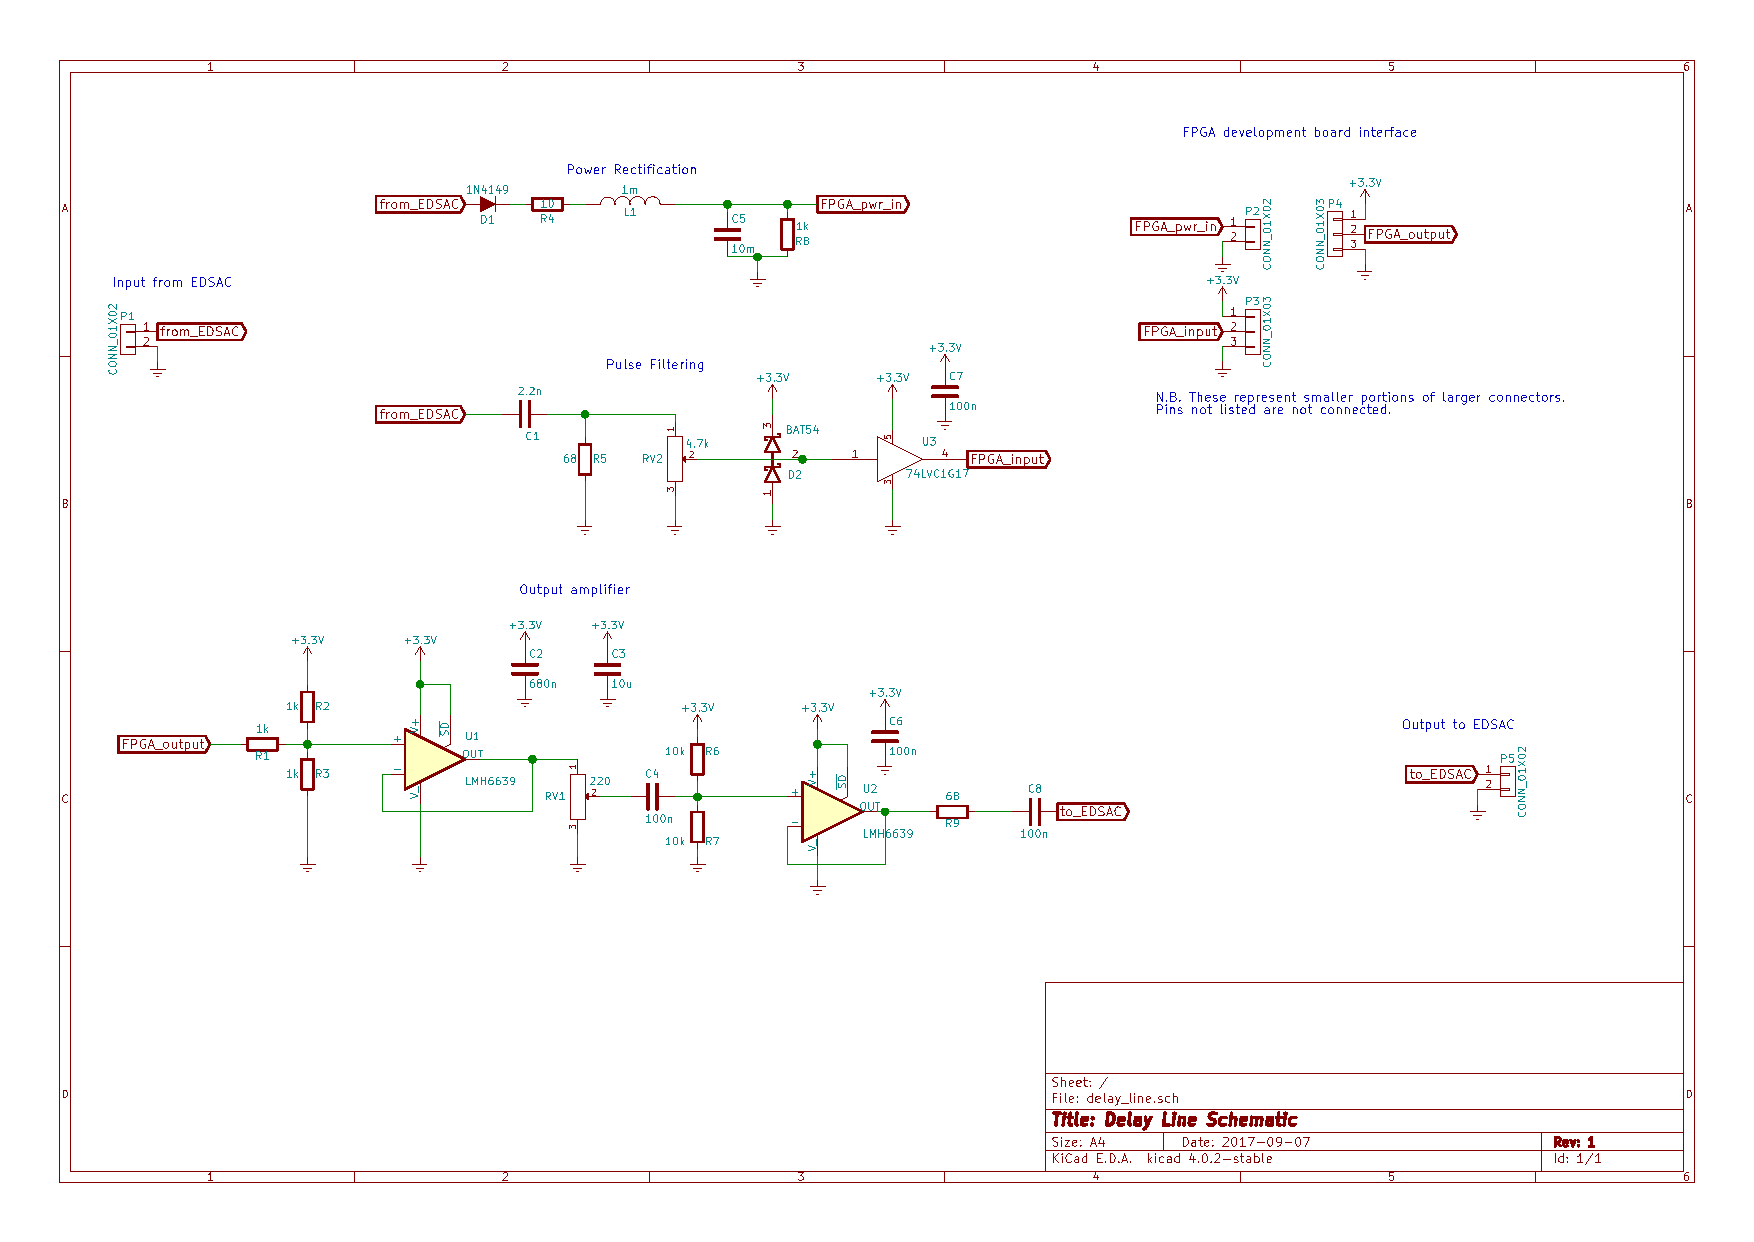
\includepdf[landscape]{figs/schematics/delay_line}
	\includepdf[landscape]{figs/schematics/test_harness}
%\end{landscape}


\chapter{\glsentryshort{hdl} verification results} \label{app:sim-wfms}
This appendix includes the the simulation waveforms resulting from verification.

The waveforms are included here since they are more clearly presented in landscape format, however they are discussed in Section \ref{sec:hdl-verif}.


\begin{landscape}

\begin{figure}[ht]
	\centering
	
	\begin{subfigure}[b]{\linewidth}
		\centering
		\includegraphics[width=\linewidth]{sim_results/delay_line/full_sim}
		\caption{Full simulation}
		\label{fig:delay-sim-full}
	\end{subfigure}
	
	\begin{subfigure}[b]{\linewidth}
		\centering
		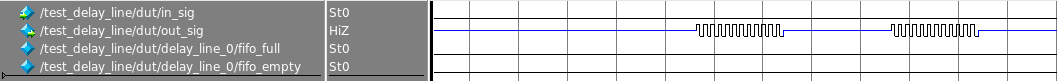
\includegraphics[width=\linewidth]{sim_results/delay_line/single_pulse}
		\caption{Simulated output of a single pulse}
		\label{fig:delay-sim-single}
	\end{subfigure}
	
	\caption{Delay line simulation results}
	\label{fig:delay-sim}
\end{figure}

\begin{figure}[ht]
	\centering
	\includegraphics[width=\linewidth]{sim_results/test_harness/full_sim}
	\caption{Full Simulation}
	\label{fig:harness-full}
\end{figure}

\end{landscape}

\end{appendices}